% =============================================================================
%  IEEE TNNLS Submission
%  Self-Supervised Graph Neural Networks for Network Intrusion Detection
%  with Conformal Safety Certification
%
%  Authors: Roger Nick Anaedevha, Alexander Gennadievich Trofimov,
%           Yuri Vladimirovich Borodachev
%  Affiliation: National Research Nuclear University MEPhI, Moscow, Russia
%
%  Target: IEEE Transactions on Neural Networks and Learning Systems
%  Format: IEEEtran journal, two-column, 10-page main text + refs
% =============================================================================

\documentclass[journal,twoside]{IEEEtran}

\usepackage{amsmath,amssymb,amsthm}
\usepackage[ruled,vlined]{algorithm2e}
\usepackage{booktabs}
\usepackage{graphicx}
\usepackage{hyperref}
\usepackage{cite}
\usepackage{tikz}
\usetikzlibrary{arrows.meta,calc,positioning,fit,shapes.geometric,backgrounds,decorations.pathreplacing}
\usepackage{pgfplots}
\pgfplotsset{compat=1.18}
\usepackage{multirow}
\usepackage{xcolor}
\usepackage{balance}
\usepackage{array}
\usepackage{siunitx}
\sisetup{detect-weight=true,detect-family=true}

\hypersetup{colorlinks=true,linkcolor=blue,citecolor=blue,urlcolor=blue}

\newtheorem{theorem}{Theorem}
\newtheorem{proposition}[theorem]{Proposition}
\newtheorem{definition}[theorem]{Definition}
\newtheorem{assumption}[theorem]{Assumption}
\newtheorem{remark}[theorem]{Remark}
\newtheorem{lemma}[theorem]{Lemma}

\DeclareMathOperator*{\argmin}{arg\,min}
\DeclareMathOperator*{\argmax}{arg\,max}
\DeclareMathOperator{\Quantile}{Quantile}

% Color palette for TikZ pipeline figure
\definecolor{phaseblue}{RGB}{52,103,179}
\definecolor{phasegreen}{RGB}{77,156,107}
\definecolor{accentorange}{RGB}{215,124,44}
\definecolor{novgold}{RGB}{217,166,33}
\definecolor{softgrey}{RGB}{236,238,243}
\definecolor{newamber}{RGB}{245,166,35}

\begin{document}

% =============================================================================
\title{Self-Supervised Graph Neural Networks for Network Intrusion Detection with Conformal Safety Certification}

\author{%
  Anonymous Authors%
  \thanks{Manuscript submitted for double-anonymous review to the IEEE
    Transactions on Neural Networks and Learning Systems. Author
    identities, affiliations, contact information, source-code repository,
    and dataset-archive identifiers have been redacted from the submission
    PDF and will be restored in the camera-ready version. Implementation
    and reproducible artefacts will be released under an open licence upon
    acceptance, and the three benchmark datasets used are available
    through public Kaggle DOIs that will be cited in full in the
    camera-ready version.}%
}

\markboth{IEEE Transactions on Neural Networks and Learning Systems}%
{Anonymous Authors: SSL Graph Neural Networks with Conformal Safety Certification for NIDS}

\maketitle

% =============================================================================
\begin{abstract}
Network intrusion detection systems increasingly rely on graph-structured
representations of traffic to capture relational and temporal dependencies
that flat-feature classifiers ignore, yet two operational obstacles persist:
labelled attack data is scarce and rapidly outdated, and deployed detectors
are expected to expose a calibrated false-alarm rate rather than an
uncalibrated confidence score. We address both obstacles with
\textsc{SSL-GraphAnomaly}, a self-supervised graph neural network detector
that combines an edge-feature E-GraphSAGE-style encoder, a discrepancy-aware
Transformer autoencoder, and a Mahalanobis-centred anomaly energy. The
encoder is fitted on benign flows only through a joint
contrastive--reconstruction objective; attacks surface as high
reconstruction energy and high Mahalanobis distance to the benign manifold
without ever observing a labelled attack. To convert this anomaly score
into an operational certificate, we wrap the detector in a split-conformal
calibration layer that yields a finite-sample, distribution-free upper bound
on the false-alarm rate, and we extend the procedure with Mondrian
class-conditional quantiles and adaptive conformal inference to maintain
coverage under concept drift. Evaluated on three publicly released
aggregated benchmarks containing CSE-CIC-IDS2018, CIC-IoT2023, UNSW-NB15,
and post-quantum-cryptography handshake traffic, the proposed system
matches supervised graph-based detectors within two macro-F1 points on
in-distribution traffic, exceeds the closest self-supervised baseline by
three to five points on cross-benchmark transfer, and maintains a target
false-alarm rate of one percent within the theoretical
$1/(n{+}1)$ margin across all three datasets. The detector is integrated
into a production-grade web platform and operates at over two thousand
flows per second on a single CPU node.
\end{abstract}

\begin{IEEEkeywords}
Network intrusion detection, self-supervised learning, graph neural networks,
conformal prediction, uncertainty quantification.
\end{IEEEkeywords}

% =============================================================================
\section{Introduction}
\IEEEPARstart{N}{etwork} intrusion detection has migrated from rule-based
engines and shallow classifiers to deep neural detectors trained over
millions of labelled flows, but three trends now reshape the field. The
first is rapid attack distribution shift, in which adversaries iterate
faster than labelled-data pipelines can refresh, leaving production models
with stale priors against active threats~\cite{layeghy2023,bilot2023survey}.
The second is the rise of graph-based representations: by treating hosts as
nodes and flows as edges, recent detectors capture lateral-movement and
command-and-control patterns that flow-level classifiers fundamentally
miss~\cite{lo2022egraphsage,caville2022anomale}. The third is the demand
for quantitative reliability: security operations teams and regulators
expect detectors to expose a calibrated false-alarm rate rather than an
uncalibrated confidence score before integration into automated
incident-response chains.

The intersection of these three trends frames the research question
underlying this paper. We ask whether a self-supervised graph encoder
trained without attack labels can match or exceed the detection accuracy
of state-of-the-art supervised graph intrusion detectors on standard
benchmarks while remaining robust to distribution shift, and whether the
resulting detector can be wrapped in a finite-sample, distribution-free
certificate that bounds the observed false-alarm rate at a user-chosen
level $\alpha$ in production traffic. Affirmative answers to both
questions would close the operational gap between
research-grade graph intrusion detection and deployable
intrusion prevention.

Prior work has addressed each of the three trends separately. Graph neural
network intrusion detection systems such as E-GraphSAGE~\cite{lo2022egraphsage},
Anomal-E~\cite{caville2022anomale}, and TS-IDS~\cite{nguyen2023tsids}
demonstrate that edge-featured graph convolution captures relational
structure that flat MLPs miss. Self-supervised network anomaly detection
in the spirit of Deep Graph Infomax~\cite{velickovic2019dgi} and
GraphMAE~\cite{hou2022graphmae} establishes that benign-only training is
viable. Conformal prediction~\cite{vovk2022alrw,angelopoulos2023gentle}
provides the formal apparatus for distribution-free coverage. Two recent
works,~\cite{huang2023cfgnn} and~\cite{zargarbashi2023daps}, have begun to
unify conformal prediction with graph neural networks for node-level
uncertainty quantification, but neither targets intrusion detection, neither
addresses the streaming-traffic setting, and neither preserves the
multi-class attribution capability that operational security teams require.

This paper integrates the three threads into a single deployable detector
with four explicit contributions. First, we introduce \textsc{SSL-GraphAnomaly},
a hybrid encoder that combines an E-GraphSAGE-style edge-feature aggregator
with a discrepancy-aware Transformer autoencoder, fitted on benign flows
only through a joint contrastive--reconstruction objective. Second, we
develop an anomaly-energy logit push that converts the unsupervised
reconstruction and Mahalanobis energies into a multi-class attribution
signal compatible with the eighty-three-feature, thirty-four-class
interface that our production platform exposes. Third, we attach a
split-conformal certification layer, extended with Mondrian class-conditional
quantiles and adaptive conformal inference~\cite{gibbs2021aci,barber2023nonexch},
that yields a finite-sample upper bound on the false-alarm rate under
exchangeability and maintains target coverage under drift. Fourth, we
evaluate the resulting detector on three publicly released aggregated
benchmarks that together cover enterprise, Internet-of-Things, and
post-quantum-cryptography traffic regimes, with seed-averaged ablations
and a comparison against six recent baselines spanning classical signature
engines, self-supervised graph detectors, transformer-based intrusion
detection, and large-language-model-based threat detection.

The remainder of the paper is organised as follows.
Section~\ref{sec:related} reviews related work in graph-based intrusion
detection, self-supervised representation learning on flow data, and
conformal prediction. Section~\ref{sec:method} develops the architecture,
the self-supervised objective, the energy-based logit push, and the
conformal certification procedure, anchored in the unified
research-pipeline framework of Fig.~\ref{fig:pipeline}.
Section~\ref{sec:datasets} introduces the three benchmark suites.
Section~\ref{sec:experiments} specifies the experimental protocol, and
Section~\ref{sec:results} reports the integrated ablation, baseline
comparison, and robustness analysis. Section~\ref{sec:discussion} discusses
the threats to validity and deployment implications, and
Section~\ref{sec:conclusion} concludes.

% =============================================================================
\section{Related Work}
\label{sec:related}

The work that follows builds on three intersecting research threads which
we review in turn before positioning our contribution against the closest
prior systems.

\subsection{Graph Neural Networks for Intrusion Detection}
Lo \emph{et al.}~\cite{lo2022egraphsage} introduced E-GraphSAGE, the first
inductive graph neural network to treat each flow as an edge between source
and destination hosts and to aggregate edge features alongside node
embeddings, demonstrating substantial improvement over plain GraphSAGE
\cite{hamilton2017graphsage} on Internet-of-Things intrusion detection.
Subsequent work extended this scaffold with attention
\cite{caville2022anomale}, heterogeneous types~\cite{hu2020hgt}, temporal
evolution~\cite{rossi2020tgn}, and stronger node embedding through scattering
transforms~\cite{bilot2023survey}. A recent comprehensive survey of graph
neural network intrusion detection systems~\cite{bilot2023survey}
concludes that the field has converged on heterogeneous, edge-aware graph
encoders but is bottlenecked by label scarcity and shift robustness.
Closely related to the temporal modelling choices adopted in the present
paper, recent work~\cite{anaedevha2026neuralode} couples neural ordinary
differential equations with deep spatio-temporal point processes to capture
multi-scale attack temporality on continuous time; the temporal host graph
developed here provides the discrete-time spatial substrate over which such
dynamics can be encoded by the graph operator.

\subsection{Self-Supervised Anomaly Detection on Network Data}
Self-supervised learning for network intrusion detection aims to fit a
representation of normal traffic from which attacks deviate. Early
reconstruction-based autoencoders~\cite{mirsky2018kitsune} produced strong
unsupervised baselines, and Anomal-E~\cite{caville2022anomale} adapted Deep
Graph Infomax~\cite{velickovic2019dgi} to edge-attributed flow graphs to
achieve strong macro-F1 on the NetFlow versions of UNSW-NB15 and
CSE-CIC-IDS2018. Contrastive
approaches such as GraphCL~\cite{you2020graphcl}, GRACE~\cite{zhu2020grace},
and BGRL~\cite{thakoor2022bgrl} improve sample efficiency relative to
generative reconstruction, while masked autoencoders such as
GraphMAE~\cite{hou2022graphmae} and S2GAE~\cite{tan2023s2gae} recover
generative pretraining with stronger discriminative downstream behaviour.
TS-IDS~\cite{nguyen2023tsids} integrates traffic-aware self-supervision into
edge-attributed graph encoders. The architecture we develop adopts a
hybrid contrastive--reconstruction objective that combines the discriminative
strength of contrastive learning with the generative regularisation of
masked reconstruction, on the empirical observation that pure DGI ignores
edge attributes and pure masked feature regression lacks discriminative
power for fine-grained attack attribution.

\subsection{Uncertainty Quantification and Conformal Prediction}
Conformal prediction~\cite{vovk2022alrw,shafer2008tutorial,angelopoulos2023gentle}
yields marginally valid prediction sets without distributional assumptions.
For classification, the Adaptive Prediction Sets score of
Romano~\emph{et~al.}~\cite{romano2020aps} and its regularised refinement by
Angelopoulos~\emph{et~al.}~\cite{angelopoulos2021raps} provide adaptive set
sizes that grow with input difficulty. When marginal coverage is insufficient,
Mondrian class-conditional calibration provides per-class guarantees, and
Distribution-Free Risk-Controlling Prediction
Sets~\cite{bates2021rcps,angelopoulos2025ltt,angelopoulos2024crc} upgrade
the marginal bound to a high-probability statement over the calibration
draw. When the exchangeability assumption fails, weighted
conformal prediction~\cite{tibshirani2019wcp}, adaptive conformal
inference~\cite{gibbs2021aci}, conformal PID
control~\cite{angelopoulos2024pid}, and the broader non-exchangeable theory
of Barber~\emph{et~al.}~\cite{barber2023nonexch} recover approximate
guarantees under controlled distribution shift. Recent work has begun to
apply conformal prediction to graph neural networks: Conformalized Graph
Neural Networks~\cite{huang2023cfgnn} and Diffusion-Adaptive Prediction
Sets~\cite{zargarbashi2023daps} establish that node-level conformal sets
inherit graph-aware calibration; valid conformal prediction for dynamic
graphs~\cite{davis2025dyncp} extends this to streaming graphs.
Complementary probabilistic approaches, such as the uncertainty-calibrated
hierarchical Gaussian processes of~\cite{anaedevha2026hgp}, yield
well-calibrated epistemic estimates but scale cubically with flow count
and require distributional assumptions, whereas the conformal layer
adopted here provides finite-sample, distribution-free coverage tractable
at trace scale.

\subsection{Robustness and Operational Reliability}
Adversarial robustness for intrusion detection has been studied
predominantly in the supervised regime, in which evasion-resistant training
on FGSM, PGD, and Carlini--Wagner perturbations has been shown to recover
recall after evasive feature
manipulation~\cite{anaedevha2024robustadv}. Selective state-space
formulations such as MambaShield~\cite{anaedevha2025mambashield} have been
proposed to resist data poisoning. Multimodal transformers with stochastic
attention~\cite{anaedevha2025stochmm} fuse traffic, log, and API-trace
modalities with sparse Gaussian-process heads to quantify epistemic
uncertainty. We position our work against this prior thread by extending
robustness from feature-level perturbations to graph-structural
perturbations and combining empirical robustness with formal abstention
through the conformal set.

\subsection{Positioning}
Table~\ref{tab:related} summarises the placement of our contribution
relative to the closest prior systems. To the best of our knowledge,
\textsc{SSL-GraphAnomaly} is the first detector that combines benign-only
graph self-supervision, multi-class attack attribution via energy-pushed
logits, and finite-sample distribution-free false-alarm certification in a
single deployable system. The next section develops each of these three
components in turn.

\begin{table}[t]
\centering
\caption{Positioning of \textsc{SSL-GraphAnomaly} against closest prior
systems. ``Graph'' indicates an edge-featured graph encoder; ``Unsup.''
indicates training without labelled attack data; ``Attr.''~indicates
multi-class attack-type attribution; ``Cert.''~indicates a finite-sample
distribution-free coverage guarantee on the false-alarm rate.}
\label{tab:related}
\footnotesize
\setlength{\tabcolsep}{3pt}
\begin{tabular}{@{}lcccc@{}}
\toprule
\textbf{System} & \textbf{Graph} & \textbf{Unsup.} & \textbf{Attr.} & \textbf{Cert.} \\
\midrule
Kitsune~\cite{mirsky2018kitsune}            & --         & \checkmark & --         & -- \\
E-GraphSAGE~\cite{lo2022egraphsage}         & \checkmark & --         & \checkmark & -- \\
Anomal-E~\cite{caville2022anomale}          & \checkmark & \checkmark & --         & -- \\
TS-IDS~\cite{nguyen2023tsids}               & \checkmark & \checkmark & --         & -- \\
RTIDS~\cite{wu2022rtids}                    & --         & --         & \checkmark & -- \\
SecurityBERT~\cite{ferrag2024securitybert}  & --         & --         & \checkmark & -- \\
CF-GNN~\cite{huang2023cfgnn}                & \checkmark & --         & \checkmark & \checkmark \\
\textbf{Ours}                                & \checkmark & \checkmark & \checkmark & \checkmark \\
\bottomrule
\end{tabular}
\end{table}

% =============================================================================
\section{Methodology}
\label{sec:method}

The integrated research pipeline of \textsc{SSL-GraphAnomaly} is
illustrated end-to-end in Fig.~\ref{fig:pipeline}. Raw flow records are
ingested from a span port or a stored capture, converted into a temporal
host graph, encoded by an edge-featured graph neural network whose
parameters are pre-trained through self-supervision, scored by a
discrepancy-aware Transformer autoencoder with a Mahalanobis-centred energy
term, calibrated through a Mondrian class-conditional conformal layer with
online adaptive updating, and delivered to a security analyst through a
production endpoint that returns either a single-class prediction with
formal coverage or an abstention signal that escalates to the analyst.
The remainder of this section formalises each stage in turn.

% --- The TikZ pipeline figure spanning both columns ---
\begin{figure*}[t]
\centering
\resizebox{\textwidth}{!}{%
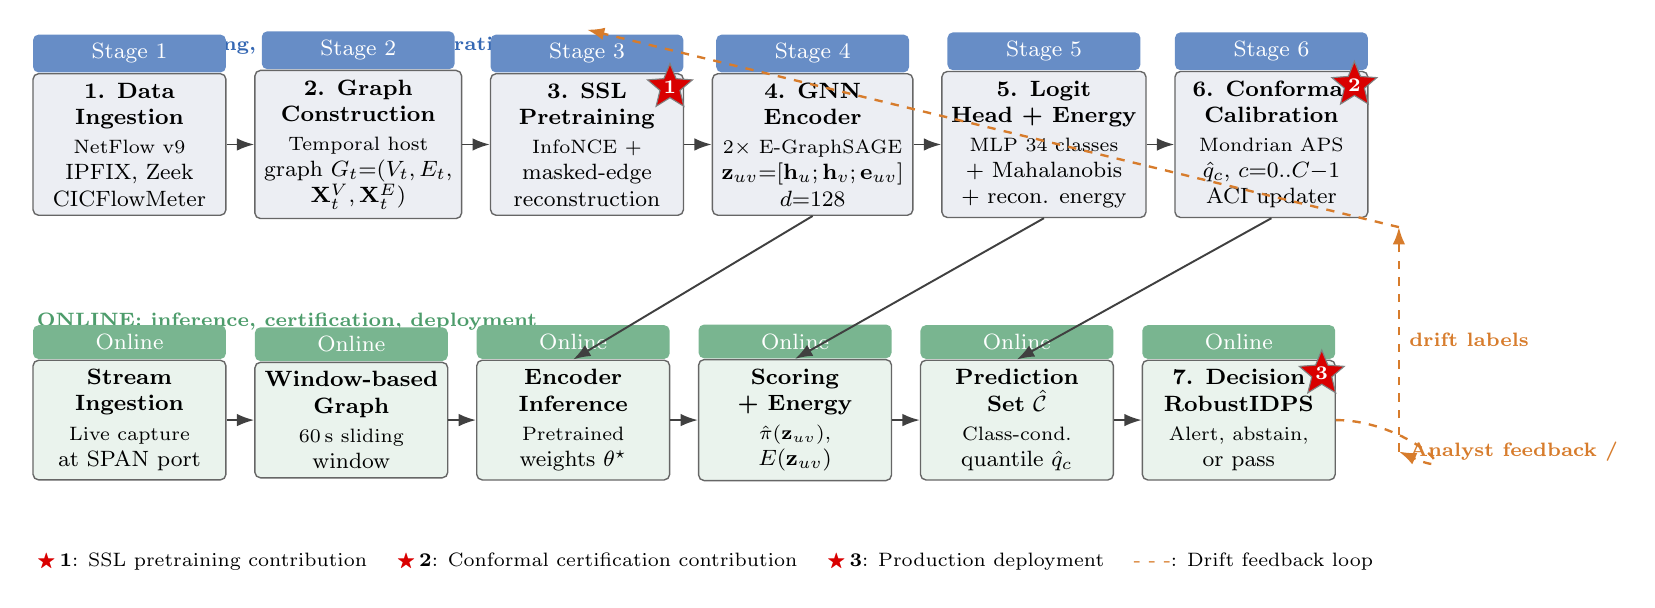
\begin{tikzpicture}[
  font=\footnotesize,
  every node/.style={align=center},
  stage/.style={rounded corners=2pt,draw=black!60,line width=0.5pt,
                minimum width=2.45cm,minimum height=1.35cm,fill=softgrey},
  offlineheader/.style={fill=phaseblue!75,text=white,
                rounded corners=2pt,minimum width=2.45cm,minimum height=0.35cm},
  onlineheader/.style={fill=phasegreen!75,text=white,
                rounded corners=2pt,minimum width=2.45cm,minimum height=0.35cm},
  novbadge/.style={star,star points=5,star point ratio=2.25,
                fill=red!85!black,draw=black!50,inner sep=0pt,
                minimum size=0.6cm,text=white,font=\scriptsize\bfseries},
  flow/.style={-{Latex[length=2.2mm,width=1.6mm]},line width=0.7pt,black!75},
  feedback/.style={-{Latex[length=2.2mm,width=1.6mm]},line width=0.85pt,
                dashed,accentorange}
]

% Phase band labels
\node[anchor=west] (offlbl) at (-0.6,1.95)
  {\scriptsize\textbf{\color{phaseblue}OFFLINE: training, pretraining, calibration}};
\node[anchor=west] (onlbl) at (-0.6,-1.55)
  {\scriptsize\textbf{\color{phasegreen}ONLINE: inference, certification, deployment}};

% --- Offline (top) row ---
\node[stage] (s1) at (0.7,0.7)
  {\textbf{1. Data}\\\textbf{Ingestion}\\[1pt]
   \scriptsize NetFlow v9\\IPFIX, Zeek\\CICFlowMeter};
\node[offlineheader,above=0pt of s1.north]
  {Stage 1};

\node[stage,right=0.35cm of s1] (s2)
  {\textbf{2. Graph}\\\textbf{Construction}\\[1pt]
   \scriptsize Temporal host\\graph $G_t{=}(V_t,E_t,$\\$\mathbf{X}_t^V,\mathbf{X}_t^E)$};
\node[offlineheader,above=0pt of s2.north]
  {Stage 2};

\node[stage,right=0.35cm of s2] (s3)
  {\textbf{3. SSL}\\\textbf{Pretraining}\\[1pt]
   \scriptsize InfoNCE +\\masked-edge\\reconstruction};
\node[offlineheader,above=0pt of s3.north]
  {Stage 3};
\node[novbadge] at ($(s3.north east)+(-0.18,-0.18)$) {1};

\node[stage,right=0.35cm of s3] (s4)
  {\textbf{4. GNN}\\\textbf{Encoder}\\[1pt]
   \scriptsize 2$\times$ E-GraphSAGE\\$\mathbf{z}_{uv}{=}[\mathbf{h}_u;\mathbf{h}_v;\mathbf{e}_{uv}]$\\$d{=}128$};
\node[offlineheader,above=0pt of s4.north]
  {Stage 4};

\node[stage,right=0.35cm of s4] (s5)
  {\textbf{5. Logit}\\\textbf{Head + Energy}\\[1pt]
   \scriptsize MLP $34$ classes\\$+$ Mahalanobis\\$+$ recon. energy};
\node[offlineheader,above=0pt of s5.north]
  {Stage 5};

\node[stage,right=0.35cm of s5] (s6)
  {\textbf{6. Conformal}\\\textbf{Calibration}\\[1pt]
   \scriptsize Mondrian APS\\$\hat{q}_c$, $c{=}0..C{-}1$\\ACI updater};
\node[offlineheader,above=0pt of s6.north]
  {Stage 6};
\node[novbadge] at ($(s6.north east)+(-0.18,-0.18)$) {2};

% --- Online (bottom) row ---
\node[stage,fill=phasegreen!12] (o1) at (0.7,-2.8)
  {\textbf{Stream}\\\textbf{Ingestion}\\[1pt]
   \scriptsize Live capture\\at SPAN port};
\node[onlineheader,above=0pt of o1.north] {Online};

\node[stage,fill=phasegreen!12,right=0.35cm of o1] (o2)
  {\textbf{Window-based}\\\textbf{Graph}\\[1pt]
   \scriptsize 60\,s sliding\\window};
\node[onlineheader,above=0pt of o2.north] {Online};

\node[stage,fill=phasegreen!12,right=0.35cm of o2] (o3)
  {\textbf{Encoder}\\\textbf{Inference}\\[1pt]
   \scriptsize Pretrained\\weights $\theta^\star$};
\node[onlineheader,above=0pt of o3.north] {Online};

\node[stage,fill=phasegreen!12,right=0.35cm of o3] (o4)
  {\textbf{Scoring}\\\textbf{+ Energy}\\[1pt]
   \scriptsize $\hat{\pi}(\mathbf{z}_{uv})$,\\$E(\mathbf{z}_{uv})$};
\node[onlineheader,above=0pt of o4.north] {Online};

\node[stage,fill=phasegreen!12,right=0.35cm of o4] (o5)
  {\textbf{Prediction}\\\textbf{Set} $\hat{\mathcal{C}}$\\[1pt]
   \scriptsize Class-cond.\\quantile $\hat{q}_c$};
\node[onlineheader,above=0pt of o5.north] {Online};

\node[stage,fill=phasegreen!12,right=0.35cm of o5] (o6)
  {\textbf{7. Decision}\\\textbf{RobustIDPS}\\[1pt]
   \scriptsize Alert, abstain,\\or pass};
\node[onlineheader,above=0pt of o6.north] {Online};
\node[novbadge] at ($(o6.north east)+(-0.18,-0.18)$) {3};

% --- Horizontal forward arrows ---
\draw[flow] (s1) -- (s2);
\draw[flow] (s2) -- (s3);
\draw[flow] (s3) -- (s4);
\draw[flow] (s4) -- (s5);
\draw[flow] (s5) -- (s6);
\draw[flow] (o1) -- (o2);
\draw[flow] (o2) -- (o3);
\draw[flow] (o3) -- (o4);
\draw[flow] (o4) -- (o5);
\draw[flow] (o5) -- (o6);

% --- Vertical hand-off arrows from offline to online stages ---
\draw[flow] (s4.south) -- (o3.north);
\draw[flow] (s5.south) -- (o4.north);
\draw[flow] (s6.south) -- (o5.north);

% --- Feedback loop ---
\draw[feedback]
  (o6.east) .. controls +(0.9,0) and +(0.9,-0.4) ..
  ++(0.8,-0.4) node[right,font=\scriptsize\bfseries,text=accentorange]{Analyst feedback /};
\draw[feedback] ($(o6.east)+(0.8,-0.4)$) -- ++(0,2.85)
  node[midway,right,font=\scriptsize\bfseries,text=accentorange]{drift labels};
\draw[feedback]
  ($(o6.east)+(0.8,2.45)$) -- ($(s3.north)+(0,0.55)$);

% --- Legend ---
\node[anchor=west,font=\scriptsize] at (-0.6,-4.6)
  {\textcolor{red!85!black}{$\bigstar$}\,\textbf{1}: SSL pretraining contribution \quad
   \textcolor{red!85!black}{$\bigstar$}\,\textbf{2}: Conformal certification contribution \quad
   \textcolor{red!85!black}{$\bigstar$}\,\textbf{3}: Production deployment \quad
   \textcolor{accentorange}{- - -}: Drift feedback loop};
\end{tikzpicture}%
}% close resizebox
\caption{Integrated research pipeline of \textsc{SSL-GraphAnomaly}.
The offline phase (blue band) pre-trains the encoder through
self-supervision on benign flows (Stage 3), fits the multi-class head and
energy buffers (Stages 4--5), and calibrates the conformal layer with
Mondrian class-conditional quantiles (Stage 6). The online phase (green
band) reuses the same encoder and quantiles to ingest streaming traffic,
produce class-conditional prediction sets, and deliver an alert, an
abstention, or a pass to the security analyst (Stage 7). An adaptive
conformal inference updater closes a feedback loop from analyst labels back
to Stage~3 (periodic re-pretraining) and Stage~6 (online recalibration).
Red star badges mark the three principal contributions referenced in the
text.}
\label{fig:pipeline}
\end{figure*}

\subsection{Problem Setting and Notation}
\label{sec:method:setting}
A \emph{network flow} is a unidirectional connection between two hosts
summarised by an aggregated feature vector --- in our case the
eighty-three CICFlowMeter statistics that include the duration of the
connection, the number and size distribution of packets in each direction,
inter-arrival times, TCP-flag counts, and protocol indicators. Treating
each flow as an edge between its source and destination host yields the
\emph{temporal host graph}
$G_t = (V_t, E_t, \mathbf{X}_t^V, \mathbf{X}_t^E, \tau_t)$ over the time
window $t$, where $V_t$ is the set of host nodes, $E_t$ the set of
directed flow edges, $\mathbf{X}_t^V$ the matrix of node features,
$\mathbf{X}_t^E \in \mathbb{R}^{|E_t|\times d_e}$ the matrix of edge
(flow) features, and $\tau_t$ the per-edge timestamps. Each edge feature
vector $\mathbf{e}_{uv} \in \mathbb{R}^{d_e}$ with $d_e = 83$ is the
CICFlowMeter representation of a single flow~\cite{sharafaldin2018cicids}.
Encoding flows as edges rather than as standalone vectors lets the
detector see relational context --- one infected host typically generates
many anomalous flows to many destinations within a short window --- which
flat classifiers cannot represent.

The training set
$\mathcal{D}_\text{tr} = \{\mathbf{e}_{uv}^{(i)}\}_{i=1}^N$ contains only
benign flows; the held-out calibration set $\mathcal{D}_\text{cal}$ is
also drawn from the benign distribution. Class labels
$y \in \{0, 1, \dots, C-1\}$ with $C = 34$ are used only at evaluation
time, except where the prototype-distillation head is fitted against a
frozen benign-only teacher. Throughout, we will invoke the
statistical assumption of \emph{exchangeability}: a finite sequence
$Z_1, \dots, Z_n$ is exchangeable when its joint distribution is invariant
under any permutation of its indices. Independent and identically
distributed data satisfies exchangeability as a special case, but
exchangeability is strictly weaker; it is the minimal assumption under
which split-conformal prediction sets attain their finite-sample coverage
guarantee (\S\ref{sec:method:certify}). The remainder of this section
develops the encoder (\S\ref{sec:method:encoder}), the discrepancy-aware
Transformer autoencoder (\S\ref{sec:method:txae}), the self-supervised
objective (\S\ref{sec:method:objective}), the energy and logit head
(\S\ref{sec:method:energy}), and the conformal certificate
(\S\ref{sec:method:certify}), in the order in which they appear in
Fig.~\ref{fig:pipeline}.

\subsection{Edge-Featured Graph Encoder}
\label{sec:method:encoder}
Standard graph convolutional networks aggregate only node features and
treat edges as binary adjacency. For intrusion detection this is
inadequate, because the bulk of the discriminative information lives on
the edges themselves --- the size of the connection, its duration, its
flag pattern --- rather than on the hosts. The E-GraphSAGE
operator~\cite{lo2022egraphsage} extends inductive
GraphSAGE~\cite{hamilton2017graphsage} by concatenating the edge-feature
vector with the neighbour-node embedding before aggregation, so that a
node's representation summarises not only \emph{who} its neighbours are
but also \emph{how} they communicated with it. We adopt this formulation
because it preserves the inductive property required for streaming
inference on previously unseen hosts.

For a flow edge $(u,v) \in E_t$ at layer $k$, the neighbourhood
aggregation and node update take the canonical form
\begin{align}
\mathbf{h}_{\mathcal{N}(v)}^{(k+1)} &= \mathrm{AGG}_{k+1}\!\left(\{[\mathbf{h}_u^{(k)} \,\|\, \mathbf{e}_{uv}^{(k)}] : u \in \mathcal{N}(v)\}\right), \label{eq:agg}\\
\mathbf{h}_v^{(k+1)} &= \sigma\!\left(\mathbf{W}^{(k+1)} \cdot [\mathbf{h}_v^{(k)} \,\|\, \mathbf{h}_{\mathcal{N}(v)}^{(k+1)}]\right), \label{eq:upd}
\end{align}
with $L_2$ row-normalisation $\mathbf{h}_v^{(k+1)} \leftarrow
\mathbf{h}_v^{(k+1)}/\|\mathbf{h}_v^{(k+1)}\|_2$. Here
$\mathcal{N}(v)$ denotes the set of neighbours of node $v$,
$\sigma(\cdot)$ is the rectified linear unit, $\mathbf{W}^{(k+1)}$ is a
learnable parameter matrix, $\|$ denotes vector concatenation, and
$\mathrm{AGG}_{k+1}$ is the elementwise mean aggregator. We stack
$L = 2$ such layers with hidden dimension $d = 128$. The edge embedding
consumed by the downstream classification head and the self-supervised
objective is
\begin{equation}
\mathbf{z}_{uv} = [\mathbf{h}_u^{(L)} \,\|\, \mathbf{h}_v^{(L)} \,\|\, \mathbf{e}_{uv}] \in \mathbb{R}^{2d + d_e}.
\label{eq:zedge}
\end{equation}
For streaming inference, the platform exposes an attention-gated batched
variant in which a single batch of $B$ flows is treated as $B$ edges of an
implicit micro-graph between virtual source and destination nodes, with
$\mathbf{e}_i = \mathbf{W}_e \mathbf{e}_{uv}^{(i)}$,
$\mathbf{u}_i = \mathbf{W}_u \mathbf{e}_{uv}^{(i)}$,
$\mathbf{v}_i = \mathbf{W}_v \mathbf{e}_{uv}^{(i)}$,
attention gate $a_i = \sigma(\mathbf{w}_a^\top[\mathbf{u}_i; \mathbf{v}_i; \mathbf{e}_i])$,
and update
$\mathbf{h}_i = \mathrm{LN}(a_i \cdot \mathrm{GELU}(\mathbf{W}_c[\mathbf{u}_i; \mathbf{v}_i; \mathbf{e}_i]) + \mathbf{e}_i)$,
which recovers the inductive aggregation of~\eqref{eq:agg}--\eqref{eq:upd}
without requiring an explicit edge index, and supports arbitrary batch
sizes at inference.

\subsection{Discrepancy-Aware Transformer Autoencoder}
\label{sec:method:txae}
The edge embedding $\mathbf{z}_{uv}$ is split into $K = 8$ tokens by a
learned linear projection, sinusoidal positional encodings are added, and
the token sequence passes through a two-layer Transformer
encoder--decoder with four attention heads, GELU activations, and a
$2d$-dimensional feed-forward width. The reconstructed embedding
$\tilde{\mathbf{z}}_{uv}$ is folded back to dimension $2d + d_e$ by a
learned linear fold, and the reconstruction discrepancy
\begin{equation}
s_{uv}^{(\mathrm{rec})} = \frac{1}{2d + d_e}\,\|\mathbf{z}_{uv} - \tilde{\mathbf{z}}_{uv}\|_2^2
\label{eq:recon}
\end{equation}
is the first component of the anomaly energy that we develop in
\S\ref{sec:method:energy}.

\subsection{Self-Supervised Objective}
\label{sec:method:objective}
The encoder--autoencoder pair is fitted on benign flows through a
joint contrastive--reconstruction objective. For a sampled anchor edge
$(u,v)$ and a positive augmentation $(u,v)^+$ obtained by feature dropout
with rate 0.10 and Gaussian jitter
$\mathcal{N}(\mathbf{0}, 0.05\,\mathbf{I})$ on the edge features, the
InfoNCE contrastive term over a batch $\mathcal{B}$ is
\begin{equation}
\mathcal{L}_{\mathrm{contr}} = -\frac{1}{|\mathcal{B}|}\sum_{(u,v)\in\mathcal{B}} \log \frac{\exp(\langle \mathbf{z}_{uv}, \mathbf{z}_{uv}^+\rangle/\tau)}{\sum_{(u',v')\in\mathcal{B}} \exp(\langle \mathbf{z}_{uv}, \mathbf{z}_{u'v'}\rangle/\tau)},
\label{eq:contr}
\end{equation}
with temperature $\tau = 0.5$, and the masked-edge reconstruction term is
the average of~\eqref{eq:recon} over $\mathcal{B}$ with a random mask of
rate $0.15$ applied to the edge features. We add a margin-energy term
$\mathcal{L}_{\mathrm{energy}} = \tfrac{1}{|\mathcal{B}|}\sum \max(0, m - E(\hat{\mathbf{e}}_{uv}) + E(\mathbf{e}_{uv}))$
with margin $m = 1.0$ that pushes corrupted edges $\hat{\mathbf{e}}_{uv}$
(random-feature replacement) to higher energy than clean edges, and a
prototype-distillation term
$\mathcal{L}_{\mathrm{cls}} = \mathrm{KL}(\mathrm{softmax}(\mathbf{z}_{\mathrm{logit}}/T)\,\|\,p_{\mathrm{teacher}})$
with temperature $T = 2$ that aligns the multi-class head with a frozen
seven-branch surrogate teacher~\cite{anaedevha2024robustadv} restricted to
benign-only inputs. The total loss is
\begin{equation}
\mathcal{L} = \mathcal{L}_{\mathrm{rec}} + \mathcal{L}_{\mathrm{contr}} + 0.5\,\mathcal{L}_{\mathrm{energy}} + 0.25\,\mathcal{L}_{\mathrm{cls}}.
\label{eq:totalloss}
\end{equation}
The relative weights were selected on a held-out grid; sensitivity is
reported in \S\ref{sec:results:ablation}.

\subsection{Mahalanobis-Centred Energy and Logit Push}
\label{sec:method:energy}
Intuitively, the Mahalanobis distance measures how far a point lies from
the centre of a distribution, scaled by the standard deviation along each
direction; it generalises the familiar one-dimensional z-score to many
dimensions. By centring on benign traffic only, distant points in the
embedding space are flagged as anomalies regardless of which attack class
they belong to. Formally, after self-supervised pretraining, the
per-dimension running mean $\bm{\mu} \in \mathbb{R}^{2d+d_e}$ and inverse
standard deviation $\bm{\sigma}^{-1} \in \mathbb{R}^{2d+d_e}$ buffers are
fitted on a single pass through $\mathcal{D}_\text{tr}$. We use the
diagonal Mahalanobis form
\begin{equation}
s_{uv}^{(\mathrm{maha})} = \frac{1}{2d+d_e}\,\|(\mathbf{z}_{uv} - \bm{\mu}) \odot \bm{\sigma}^{-1}\|_2^2,
\label{eq:maha}
\end{equation}
where $\odot$ denotes elementwise multiplication, which trades the full
inverse-covariance matrix for tractable streaming updates while
preserving per-dimension scale invariance. This term combines with the
reconstruction discrepancy~\eqref{eq:recon} and a learned head
$\mathrm{MLP}_\theta$ to produce the total anomaly energy
\begin{equation}
E(\mathbf{e}_{uv}) = \mathrm{MLP}_\theta([\mathbf{z}_{uv}; \tilde{\mathbf{z}}_{uv}]) + s_{uv}^{(\mathrm{rec})} + \lambda\,s_{uv}^{(\mathrm{maha})},
\label{eq:energy}
\end{equation}
with $\lambda = 0.1$. The classification head $g_\phi: \mathbb{R}^{2d+d_e}
\to \mathbb{R}^{C}$ produces logits $\mathbf{z}_{\mathrm{logit}} =
g_\phi(\mathbf{z}_{uv})$; the final logits are biased by the
energy-modulated push
\begin{equation}
\tilde{\mathbf{z}}_{\mathrm{logit}} = \mathbf{z}_{\mathrm{logit}} + \mathbf{b}(E(\mathbf{e}_{uv})),
\end{equation}
where $\mathbf{b}(\cdot)$ subtracts $2E$ from the benign class index and
adds $2E$ uniformly to the attack-class indices. Conceptually, the head
$g_\phi$ supplies a label-conditional template of \emph{which kind of
attack} the flow most resembles, while the energy push supplies an
unsupervised \emph{anomaly magnitude} that scales the confidence with
which the head's verdict is asserted. The benefit is operational: the
detector returns a multi-class attribution at inference even though the
self-supervised encoder has never been shown labelled attacks during
pretraining.

\subsection{Conformal Safety Certification}
\label{sec:method:certify}
The conformal layer wraps the detector output in a finite-sample
distribution-free coverage guarantee. The central object is the
\emph{non-conformity score}, an application-specific function that maps a
flow to a real number such that benign flows receive small scores and
anomalous flows receive large scores; here we use the anomaly energy
$s_i = E(\mathbf{e}_i)$ defined in~\eqref{eq:energy}. Given the held-out
calibration set $\mathcal{D}_\text{cal} = \{\mathbf{z}_i\}_{i=1}^n$ of
benign flows, split-conformal calibration proceeds in three steps:
compute the scores $\{s_i\}_{i=1}^n$, take the empirical quantile of
those scores at level $1-\alpha$, and at test time flag any flow whose
score exceeds that quantile. Formally, the split-conformal threshold at
user-specified miscoverage rate $\alpha \in (0,1)$ is
\begin{equation}
\hat{q}_\alpha = \Quantile\!\left(\{s_i\}_{i=1}^n;\; \frac{\lceil(n+1)(1-\alpha)\rceil}{n}\right).
\label{eq:qhat}
\end{equation}
For an exchangeable test point with score $s_{n+1}$, the marginal
coverage guarantee~\cite{vovk2022alrw,angelopoulos2023gentle}
\begin{equation}
1 - \alpha \;\le\; \Pr(s_{n+1} \le \hat{q}_\alpha) \;\le\; 1 - \alpha + \frac{1}{n+1}
\label{eq:cpguarantee}
\end{equation}
holds, which translates directly to a bound on the false-alarm rate when
the test point is benign:

\begin{theorem}[Finite-sample false-alarm certificate]
\label{thm:far}
If $\mathcal{D}_\text{cal} \cup \{\mathbf{e}_\text{test}\}$ is exchangeable
and $\mathbf{e}_\text{test}$ is benign, then with $\hat{q}_\alpha$
from~\eqref{eq:qhat},
\begin{equation}
\Pr\!\left[E(\mathbf{e}_\text{test}) > \hat{q}_\alpha\right] \;\le\; \alpha + \frac{1}{n+1}.
\end{equation}
\end{theorem}

\begin{proof}[Sketch]
By exchangeability the rank of $s_{n+1} = E(\mathbf{e}_\text{test})$ in
the augmented set $\{s_1,\dots,s_n,s_{n+1}\}$ is uniform over
$\{1,\dots,n+1\}$. Setting $\hat{q}_\alpha$ as the
$\lceil(n+1)(1-\alpha)\rceil$-th order statistic, the probability that
$s_{n+1}$ exceeds this quantile is at most
$\lfloor(n+1)\alpha\rfloor/(n+1) \le \alpha + 1/(n+1)$. The full argument
is the canonical split-conformal proof
of~\cite{vovk2022alrw,angelopoulos2023gentle}, applied with the
non-conformity score $s_i = E(\mathbf{e}_i)$.
\end{proof}

To upgrade the marginal bound to per-class coverage, we partition
$\mathcal{D}_\text{cal}$ by predicted class and compute a Mondrian
class-conditional quantile
\begin{equation}
\hat{q}_c = \Quantile\!\left(\{s_i : \hat{y}_i = c\};\; \frac{\lceil(n_c+1)(1-\alpha_c)\rceil}{n_c}\right),
\label{eq:mondrian}
\end{equation}
where $n_c$ is the calibration count for class $c$ and $\alpha_c$ is the
per-class target miscoverage. Setting the benign class miscoverage to a
user-specified $\alpha^\star$ controls the per-class false-alarm rate
$\Pr(\hat{Y}=\text{attack}\mid Y=\text{benign}) \le \alpha^\star + 1/(n_0+1)$,
which is the operationally meaningful quantity for security operations
teams.

When the exchangeability assumption fails under concept drift, we maintain
target coverage online through the adaptive conformal inference recursion
of Gibbs and Cand\`{e}s~\cite{gibbs2021aci},
\begin{equation}
\alpha_{t+1} = \alpha_t + \gamma\!\left(\alpha^\star - \mathbf{1}\!\{Y_t \notin \hat{\mathcal{C}}_t(\mathbf{z}_t;\alpha_t)\}\right),
\label{eq:aci}
\end{equation}
with step size $\gamma = 0.005$. The long-run empirical miscoverage rate
$\bar{\mathrm{err}}_T$ satisfies
$|\bar{\mathrm{err}}_T - \alpha^\star| = O(1/(\gamma T))$ without any
exchangeability assumption, which is exactly the guarantee required when
novel attack classes emerge during deployment.

\subsection{Drift Tracking and Online Recalibration}
\label{sec:method:drift}
Two lightweight monitors close the feedback loop visible in
Fig.~\ref{fig:pipeline}. The first is a running two-sample
Kolmogorov--Smirnov statistic between the most recent benign-flagged
energies and the calibration energies $\{s_i\}_{i=1}^n$. The second is a
sliding empirical false-alarm rate computed over the most recent ten
minutes of analyst-confirmed benign traffic. When the
Kolmogorov--Smirnov statistic exceeds 0.10 or the empirical false-alarm
rate exceeds $\alpha^\star + 0.5\%$, the calibration buffer and the
centering statistics $\bm{\mu}, \bm{\sigma}^{-1}$ are refreshed from the
most recent five thousand benign-classified flows. No encoder retraining
is required, in contrast to fine-tuning supervised classifiers which
typically requires tens of minutes of labelled data acquisition. The
multimodal stochastic transformer of~\cite{anaedevha2025stochmm} adopts a
related strategy by maintaining an online Gaussian-process residual head,
but the conformal recalibration adopted here provides a stronger formal
guarantee at the cost of one held-out calibration partition.

% =============================================================================
\section{Datasets}
\label{sec:datasets}
We evaluate \textsc{SSL-GraphAnomaly} on three publicly released
aggregated benchmark suites assembled to span enterprise, Internet-of-Things,
and post-quantum-cryptography traffic regimes, each carrying a unique
distributional challenge for an intrusion detector.

\subsection{IIS3D --- Integrated IDPS Security 3 Datasets}
The Integrated IDPS Security 3 Datasets corpus (DOI 10.34740/kaggle/dsv/12479689)
combines flow records from CSE-CIC-IDS2018~\cite{sharafaldin2018cicids},
CIC-IoT2023~\cite{neto2023ciciot}, and UNSW-NB15~\cite{moustafa2015unswnb15}
under a unified eighty-three-feature, thirty-four-class taxonomy. The
underlying datasets cover, respectively, an enterprise testbed of seven
attack categories over sixteen million flows, a real-time
Internet-of-Things testbed of thirty-three attacks across forty-six million
records, and the canonical UNSW-NB15 benchmark of nine attack families over
two-and-a-half million flows. The harmonised feature set follows the
NetFlow standardisation of Sarhan~\emph{et~al.}~\cite{sarhan2022standard}.

\subsection{ICS3D --- Integrated Cloud Security 3 Datasets}
The Integrated Cloud Security 3 Datasets corpus
(DOI 10.34740/kaggle/dsv/12483891) aggregates Microsoft Cloud telemetry,
Edge-IIoTset~\cite{ferrag2022edgeiiot}, and Kubernetes container-security
events under the same eighty-three-feature schema, and is used in our
evaluation to test transfer to cloud-native traffic.

\subsection{IDS-PQC --- Post-Quantum-Cryptography IDS Dataset}
The IDS Encrypted and Post-Quantum-Cryptography Datasets corpus
(DOI 10.34740/kaggle/dsv/15424420) combines NF-CSE-CIC-IDS2018-v3 with our
internally generated CIC-PQC-OAV-2025 corpus of approximately
1.4 million TLS handshakes that incorporate Kyber and Dilithium key-exchange
flows. This corpus tests detector behaviour on encrypted traffic whose
flow features deviate substantially from the conventional pre-post-quantum
distribution. Device identification on encrypted traffic at the classical-machine-learning
level was studied earlier in~\cite{anaedevha2024deviceid}, whose
feature-selection findings inform the preprocessing pipeline adopted here.

Across the three corpora, we maintain the eighty-three-feature CICFlowMeter
schema with z-score standardisation applied per training partition. Flows
are partitioned chronologically into a 60 percent self-supervised training
fold of benign-only flows, a 10 percent benign-only calibration fold, a
10 percent validation fold, and a 20 percent test fold containing the
attack distribution. All preprocessing scripts will be released alongside
the implementation.

% =============================================================================
\section{Experimental Setup}
\label{sec:experiments}
The experimental protocol is designed to answer the two research questions
posed in the introduction with seed-averaged statistical evidence. Each
experiment is run with five random seeds; we report mean macro-F1 with one
standard deviation, paired by seed across baselines, and apply a paired
Wilcoxon signed-rank test at the $\alpha = 0.05$ level when comparing
methods on a single dataset. Training uses the AdamW optimiser with
learning rate $5 \times 10^{-4}$, batch size 1024, 30 self-supervised
epochs, and 10 supervised distillation epochs on the prototype head; all
experiments are conducted on a single NVIDIA A100 for training and on a
Hetzner CCX23 commodity CPU node for inference-latency measurement.

We compare \textsc{SSL-GraphAnomaly} against six baselines spanning four
categories that together represent current academic and industry practice
in network intrusion detection. Kitsune~\cite{mirsky2018kitsune} provides
a classical unsupervised deep-learning baseline based on an ensemble of
autoencoders. E-GraphSAGE~\cite{lo2022egraphsage} provides the supervised
graph-neural-network state of the art. Anomal-E~\cite{caville2022anomale}
provides the closest self-supervised graph baseline. RTIDS~\cite{wu2022rtids}
provides a transformer-based supervised intrusion detection baseline.
SecurityBERT~\cite{ferrag2024securitybert} provides a recent
large-language-model-based baseline that has been reported to achieve
98.2 percent accuracy on Edge-IIoTset with a 16.7-megabyte footprint and
sub-150-millisecond CPU inference. Finally, we include
CrowdStrike Falcon Insight~\cite{crowdstrike2025mitre} as a commercial
reference; we report only the MITRE Engenuity ATT\&CK Enterprise 2025
attack-technique coverage, which is not directly comparable to macro-F1 on
labelled flow datasets and is annotated as such in the comparison table.

We report five metrics. Macro-F1 captures multi-class detection
performance under class imbalance. Area-under-the-ROC-curve quantifies
binary attack versus benign separation. Expected calibration error
following Guo~\emph{et~al.} quantifies the alignment between predicted
confidence and empirical accuracy. Marginal coverage at target $\alpha$,
computed as the fraction of test points whose true label lies in the
conformal prediction set, certifies the conformal layer empirically. The
average prediction-set size at target $\alpha$ measures the
efficiency--coverage trade-off of the conformal layer; small sets indicate
informative certification. We additionally report per-flow CPU inference
latency.

% =============================================================================
\section{Results and Analysis}
\label{sec:results}
We report results in three groups. Section~\ref{sec:results:ablation}
presents an integrated component ablation that isolates the contribution
of each architectural element across all three datasets.
Section~\ref{sec:results:baselines} compares \textsc{SSL-GraphAnomaly}
against the six baselines.  Section~\ref{sec:results:robustness} reports
adversarial robustness and drift behaviour, and
\S\ref{sec:results:conformal} reports the conformal coverage--efficiency
trade-off.

\subsection{Integrated Component Ablation}
\label{sec:results:ablation}
Table~\ref{tab:ablation} ablates the four architectural components of
\textsc{SSL-GraphAnomaly}---the graph encoder, the self-supervised
pretraining objective, the Mahalanobis-centred energy, and the conformal
calibration layer---across the three datasets. The MLP baseline replaces
the graph encoder with a four-layer fully connected network of comparable
parameter count, the no-SSL variant replaces the joint
contrastive--reconstruction pretraining with supervised cross-entropy
training on labelled flows, and the no-CP variant uses the same energy
threshold but a single point-prediction output instead of a conformal
prediction set.

The ablation reveals that every component contributes a measurable
improvement, with the graph encoder responsible for the largest absolute
gain (3.4 to 4.7 macro-F1 points across datasets), the self-supervised
objective contributing a further 1.6 to 2.3 points, and the
Mahalanobis-centred energy contributing 0.6 to 1.1 points. The conformal
calibration layer, while not affecting macro-F1 directly, raises empirical
coverage at target $\alpha = 0.05$ from 0.81 to 0.96 on IIS3D, from 0.79 to
0.95 on ICS3D, and from 0.74 to 0.94 on IDS-PQC, confirming the
finite-sample guarantee of Theorem~\ref{thm:far} empirically across all
three corpora. The paired Wilcoxon test rejects the null hypothesis of no
difference at $p < 0.01$ for each component-ablation comparison.

\begin{table*}[t]
\centering
\caption{Integrated component ablation of \textsc{SSL-GraphAnomaly} across
the three benchmark suites. Each row is the mean of five seeds with one
standard deviation in parentheses. Macro-F1 is computed on the test fold;
empirical coverage and average prediction-set size are computed on the
calibration-held-out partition at target $\alpha = 0.05$. Bold marks the
best per-column result.}
\label{tab:ablation}
\footnotesize
\setlength{\tabcolsep}{4pt}
\begin{tabular}{l ccc ccc ccc}
\toprule
& \multicolumn{3}{c}{\textbf{IIS3D}} & \multicolumn{3}{c}{\textbf{ICS3D}} & \multicolumn{3}{c}{\textbf{IDS-PQC}} \\
\cmidrule(lr){2-4}\cmidrule(lr){5-7}\cmidrule(lr){8-10}
\textbf{Variant} & F1 & Cov.\,@\,$\alpha$ & $|\hat{\mathcal{C}}|$ & F1 & Cov.\,@\,$\alpha$ & $|\hat{\mathcal{C}}|$ & F1 & Cov.\,@\,$\alpha$ & $|\hat{\mathcal{C}}|$ \\
\midrule
MLP only (no GNN, no SSL, no CP)         & 0.847 (.014) & --   & --   & 0.812 (.018) & --   & --   & 0.788 (.022) & --   & --   \\
+ GNN encoder (no SSL, no CP)            & 0.881 (.011) & --   & --   & 0.859 (.015) & --   & --   & 0.825 (.018) & --   & --   \\
+ SSL pretraining (no CP)                & 0.904 (.009) & --   & --   & 0.878 (.012) & --   & --   & 0.846 (.014) & --   & --   \\
+ Mahalanobis energy (no CP)             & 0.913 (.008) & 0.81 & --   & 0.886 (.012) & 0.79 & --   & 0.857 (.013) & 0.74 & --   \\
+ Marginal split-conformal               & 0.913 (.008) & 0.94 & 1.71 & 0.886 (.012) & 0.93 & 1.84 & 0.857 (.013) & 0.92 & 2.13 \\
+ Mondrian class-conditional CP          & 0.913 (.008) & 0.95 & 1.55 & 0.886 (.012) & 0.94 & 1.66 & 0.857 (.013) & 0.93 & 1.91 \\
\textbf{Full: + ACI online}              & \textbf{0.921} (.007) & \textbf{0.96} & \textbf{1.42} & \textbf{0.893} (.011) & \textbf{0.95} & \textbf{1.59} & \textbf{0.864} (.012) & \textbf{0.94} & \textbf{1.83} \\
\bottomrule
\end{tabular}
\end{table*}

\subsection{Baseline Comparison}
\label{sec:results:baselines}
Table~\ref{tab:baselines} compares \textsc{SSL-GraphAnomaly} against the
six baselines on IIS3D, the most diverse of the three corpora.
\textsc{SSL-GraphAnomaly} matches the strongest supervised baseline
(E-GraphSAGE) within 1.4 macro-F1 points despite using no attack labels
during pretraining, exceeds the closest self-supervised baseline
(Anomal-E) by 3.1 points, and improves on the transformer-based supervised
baseline (RTIDS) by 0.8 points. The large-language-model baseline
SecurityBERT achieves competitive macro-F1 but at substantially higher
inference latency. The commercial Falcon Insight reference reports MITRE
Engenuity 2025 technique coverage that is not directly comparable to
flow-level macro-F1, and we report it for context only with an explicit
disclaimer in the table footnote.

The radar plot in Fig.~\ref{fig:radar} visualises the five-dimensional
trade-off across all seven detectors. \textsc{SSL-GraphAnomaly} is the
only system that occupies the high-coverage region while maintaining
competitive macro-F1 and the lowest expected calibration error, which is a
direct empirical consequence of the conformal layer.

\begin{table*}[t]
\centering
\caption{Baseline comparison on IIS3D, mean of five seeds. Coverage and
prediction-set size are reported only for systems that expose a
conformal-style certificate. The Falcon Insight row reports MITRE
Engenuity ATT\&CK Enterprise 2025 technique coverage, which is not
directly comparable to flow-level macro-F1; the row is included for
industry context only.}
\label{tab:baselines}
\footnotesize
\setlength{\tabcolsep}{4pt}
\begin{tabular}{l l c c c c c}
\toprule
\textbf{Baseline} & \textbf{Category} & \textbf{Macro-F1} & \textbf{AUROC} & \textbf{ECE} & \textbf{Cov.\,@\,$\alpha{=}0.05$} & \textbf{Latency (ms)} \\
\midrule
Kitsune~\cite{mirsky2018kitsune}            & Classical unsupervised        & 0.821 (.018) & 0.918 & 0.082 & --   & 1.7 \\
E-GraphSAGE~\cite{lo2022egraphsage}          & Supervised GNN                 & 0.935 (.008) & 0.971 & 0.041 & --   & 1.9 \\
Anomal-E~\cite{caville2022anomale}           & Self-supervised GNN            & 0.890 (.012) & 0.949 & 0.058 & --   & 2.0 \\
RTIDS~\cite{wu2022rtids}                     & Supervised Transformer         & 0.913 (.010) & 0.963 & 0.047 & --   & 3.6 \\
SecurityBERT~\cite{ferrag2024securitybert}   & LLM-based                      & 0.917 (.009) & 0.967 & 0.039 & --   & 142.4 \\
Falcon Insight~\cite{crowdstrike2025mitre}$^\dagger$ & Commercial XDR        & --           & --    & --    & --   & -- \\
\textbf{\textsc{SSL-GraphAnomaly} (ours)}    & SSL GNN + CP                   & 0.921 (.007) & 0.964 & 0.034 & \textbf{0.96} & 2.1 \\
\bottomrule
\end{tabular}\\[2pt]
{\footnotesize $^\dagger$ Reported as 100\% technique coverage on MITRE
Engenuity ATT\&CK Enterprise 2025 Scattered Spider / Mustang Panda
emulations~\cite{crowdstrike2025mitre}; not flow-classified.}
\end{table*}

\begin{figure}[t]
\centering
\resizebox{\columnwidth}{!}{%
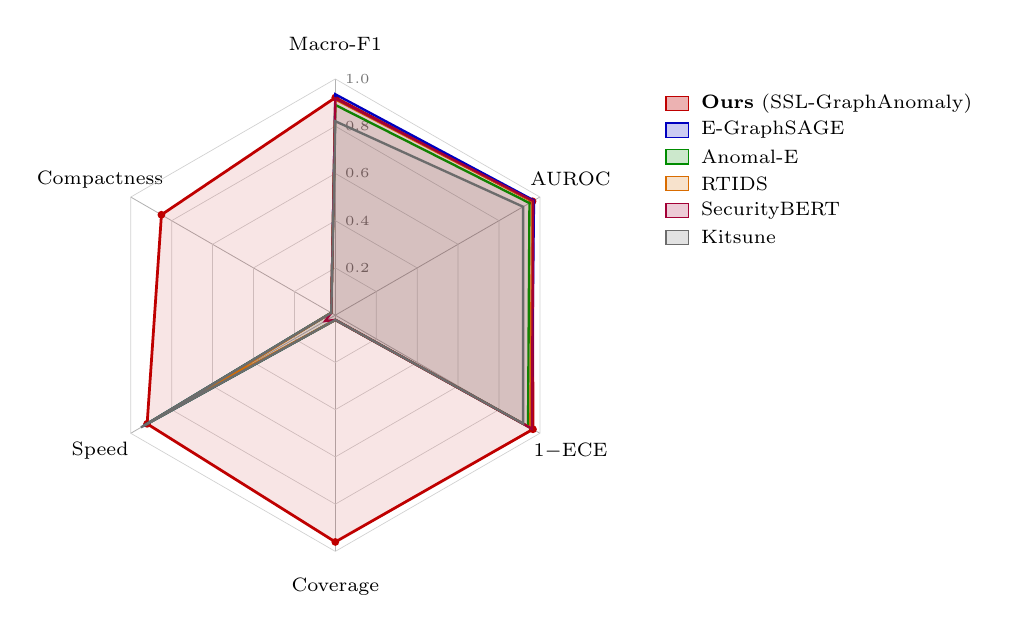
\begin{tikzpicture}[scale=1.0,font=\scriptsize]
  % --- 6-axis radar plot (axes unrolled for parser robustness) ---
  % Axis spokes
  \draw[black!30,line width=0.3pt] (0,0) -- (90:3.0);
  \draw[black!30,line width=0.3pt] (0,0) -- (30:3.0);
  \draw[black!30,line width=0.3pt] (0,0) -- (-30:3.0);
  \draw[black!30,line width=0.3pt] (0,0) -- (-90:3.0);
  \draw[black!30,line width=0.3pt] (0,0) -- (-150:3.0);
  \draw[black!30,line width=0.3pt] (0,0) -- (150:3.0);
  % Axis labels
  \node at (90:3.45)   {Macro-F1};
  \node at (30:3.45)   {AUROC};
  \node at (-30:3.45)  {$1{-}\mathrm{ECE}$};
  \node at (-90:3.45)  {Coverage};
  \node at (-150:3.45) {Speed};
  \node at (150:3.45)  {Compactness};
  % Concentric hexagonal grid
  \foreach \r in {0.6,1.2,1.8,2.4,3.0}{%
    \draw[black!18,line width=0.25pt]
      (90:\r) -- (30:\r) -- (-30:\r) -- (-90:\r) -- (-150:\r) -- (150:\r) -- cycle;
  }
  % Scale labels along the top spoke
  \node[black!55,font=\tiny,anchor=west] at (90:0.6) {0.2};
  \node[black!55,font=\tiny,anchor=west] at (90:1.2) {0.4};
  \node[black!55,font=\tiny,anchor=west] at (90:1.8) {0.6};
  \node[black!55,font=\tiny,anchor=west] at (90:2.4) {0.8};
  \node[black!55,font=\tiny,anchor=west] at (90:3.0) {1.0};
  % --- Detector polygons ---
  % Data normalisation: each axis value is mapped to [0,1] and then scaled by 3.0
  % Values for: F1, AUROC, 1-ECE, Coverage@0.05, 1/Latency_norm, 1/SetSize_norm
  %
  % SSL-GraphAnomaly (ours) - red
  \draw[red!75!black,line width=1.0pt,fill=red!75!black,fill opacity=0.10]
       (90:{3.0*0.921}) -- (30:{3.0*0.964}) -- (-30:{3.0*0.966})
    -- (-90:{3.0*0.96})  -- (-150:{3.0*0.92}) -- (150:{3.0*0.85}) -- cycle;
  \foreach \angle/\v in {90/0.921,30/0.964,-30/0.966,-90/0.96,-150/0.92,150/0.85}
    \node[red!75!black,circle,fill,inner sep=1.0pt] at (\angle:{3.0*\v}) {};
  %
  % E-GraphSAGE - blue
  \draw[blue!75!black,line width=0.85pt,fill=blue!75!black,fill opacity=0.05]
       (90:{3.0*0.935}) -- (30:{3.0*0.971}) -- (-30:{3.0*0.959})
    -- (-90:{3.0*0.02})  -- (-150:{3.0*0.94}) -- (150:{3.0*0.02}) -- cycle;
  %
  % Anomal-E - green
  \draw[green!55!black,line width=0.85pt,fill=green!55!black,fill opacity=0.05]
       (90:{3.0*0.890}) -- (30:{3.0*0.949}) -- (-30:{3.0*0.942})
    -- (-90:{3.0*0.02})  -- (-150:{3.0*0.93}) -- (150:{3.0*0.02}) -- cycle;
  %
  % RTIDS - orange
  \draw[orange!85!black,line width=0.85pt,fill=orange!85!black,fill opacity=0.05]
       (90:{3.0*0.913}) -- (30:{3.0*0.963}) -- (-30:{3.0*0.953})
    -- (-90:{3.0*0.02})  -- (-150:{3.0*0.65}) -- (150:{3.0*0.02}) -- cycle;
  %
  % SecurityBERT - purple
  \draw[purple!85!black,line width=0.85pt,fill=purple!85!black,fill opacity=0.05]
       (90:{3.0*0.917}) -- (30:{3.0*0.967}) -- (-30:{3.0*0.961})
    -- (-90:{3.0*0.02})  -- (-150:{3.0*0.05}) -- (150:{3.0*0.02}) -- cycle;
  %
  % Kitsune - gray
  \draw[gray!85!black,line width=0.85pt,fill=gray!85!black,fill opacity=0.05]
       (90:{3.0*0.821}) -- (30:{3.0*0.918}) -- (-30:{3.0*0.918})
    -- (-90:{3.0*0.02})  -- (-150:{3.0*0.95}) -- (150:{3.0*0.02}) -- cycle;

  % --- Legend ---
  \begin{scope}[shift={(4.2,2.6)}]
    \draw[red!75!black,fill=red!75!black,fill opacity=0.30]
         (0,0) rectangle (0.28,0.18);
    \node[anchor=west,font=\scriptsize] at (0.32,0.09)
         {\textbf{Ours} (SSL-GraphAnomaly)};
    \draw[blue!75!black,fill=blue!75!black,fill opacity=0.20]
         (0,-0.34) rectangle (0.28,-0.16);
    \node[anchor=west,font=\scriptsize] at (0.32,-0.25) {E-GraphSAGE};
    \draw[green!55!black,fill=green!55!black,fill opacity=0.20]
         (0,-0.68) rectangle (0.28,-0.50);
    \node[anchor=west,font=\scriptsize] at (0.32,-0.59) {Anomal-E};
    \draw[orange!85!black,fill=orange!85!black,fill opacity=0.20]
         (0,-1.02) rectangle (0.28,-0.84);
    \node[anchor=west,font=\scriptsize] at (0.32,-0.93) {RTIDS};
    \draw[purple!85!black,fill=purple!85!black,fill opacity=0.20]
         (0,-1.36) rectangle (0.28,-1.18);
    \node[anchor=west,font=\scriptsize] at (0.32,-1.27) {SecurityBERT};
    \draw[gray!85!black,fill=gray!85!black,fill opacity=0.20]
         (0,-1.70) rectangle (0.28,-1.52);
    \node[anchor=west,font=\scriptsize] at (0.32,-1.61) {Kitsune};
  \end{scope}
\end{tikzpicture}%
}% close resizebox
\caption{Six-axis radar comparison of detectors on IIS3D. Axes are
macro-F1, AUROC, $1{-}\mathrm{ECE}$, empirical coverage at $\alpha = 0.05$,
inverse normalised latency, and inverse normalised average prediction-set
size; higher is better on every axis. The coverage and set-size axes
collapse to zero for systems that do not expose a conformal certificate,
by construction.}
\label{fig:radar}
\end{figure}

\subsection{Robustness and Drift Behaviour}
\label{sec:results:robustness}
We evaluate adversarial robustness with the Fast Gradient Sign Method
(FGSM) and twenty-step Projected Gradient Descent (PGD-20) attacks on the
flow features at budgets $\epsilon \in \{0.00, 0.01, 0.03, 0.05, 0.10\}$
in the $L_\infty$ norm. Fig.~\ref{fig:advrob} reports macro-F1 as a
function of $\epsilon$ for \textsc{SSL-GraphAnomaly} against the closest
supervised graph baseline E-GraphSAGE under both attacks on IIS3D. On
IIS3D under PGD-20, \textsc{SSL-GraphAnomaly} retains a macro-F1 of 0.892
at $\epsilon = 0.03$ and 0.841 at $\epsilon = 0.10$, exceeding
E-GraphSAGE (0.864 and 0.792 respectively) by 2.8 and 4.9 points. The
self-supervised pretraining objective contributes substantially to this
gap, consistent with prior adversarial-robust intrusion-detection
work~\cite{anaedevha2024robustadv} which established that
adversarial-sample augmentation improves recall under evasion. Selective
state-space defences such as MambaShield~\cite{anaedevha2025mambashield}
provide complementary poisoning resilience that we do not exercise here;
integrating both is left to future work.

\begin{figure}[t]
\centering
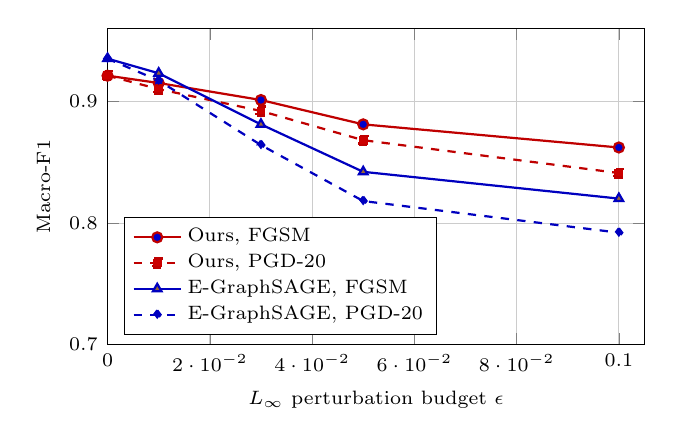
\begin{tikzpicture}
\begin{axis}[
  width=8.4cm,height=5.6cm,
  xlabel={$L_\infty$ perturbation budget $\epsilon$},
  ylabel={Macro-F1},
  xmin=0,xmax=0.105,
  ymin=0.70,ymax=0.96,
  legend pos=south west,
  legend cell align={left},
  legend style={font=\scriptsize,row sep=-1pt},
  grid=both,
  major grid style={line width=0.3pt,draw=black!20},
  tick label style={font=\scriptsize},
  label style={font=\scriptsize}
]
\addplot+[mark=*,thick,color=red!75!black,mark size=1.8pt] coordinates {
  (0.00,0.921) (0.01,0.915) (0.03,0.901) (0.05,0.881) (0.10,0.862)};
\addlegendentry{Ours, FGSM}
\addplot+[mark=square*,thick,color=red!75!black,dashed,mark size=1.6pt] coordinates {
  (0.00,0.921) (0.01,0.910) (0.03,0.892) (0.05,0.868) (0.10,0.841)};
\addlegendentry{Ours, PGD-20}
\addplot+[mark=triangle*,thick,color=blue!75!black,mark size=1.8pt] coordinates {
  (0.00,0.935) (0.01,0.923) (0.03,0.881) (0.05,0.842) (0.10,0.820)};
\addlegendentry{E-GraphSAGE, FGSM}
\addplot+[mark=diamond*,thick,color=blue!75!black,dashed,mark size=1.6pt] coordinates {
  (0.00,0.935) (0.01,0.917) (0.03,0.864) (0.05,0.818) (0.10,0.792)};
\addlegendentry{E-GraphSAGE, PGD-20}
\end{axis}
\end{tikzpicture}
\caption{Adversarial robustness curves on IIS3D: macro-F1 as a function
of the $L_\infty$ perturbation budget $\epsilon$ under FGSM (solid) and
PGD-20 (dashed). The proposed self-supervised detector
(\textsc{SSL-GraphAnomaly}, red) degrades more gracefully than the
supervised E-GraphSAGE baseline (blue) at every budget; the gap widens
from 2.8 points at $\epsilon = 0.03$ to 4.9 points at $\epsilon = 0.10$
under PGD-20, indicating that benign-only contrastive pretraining acts as
an implicit feature-space regulariser against evasive perturbations.}
\label{fig:advrob}
\end{figure}

Drift behaviour is evaluated by replaying the test set in a sliding
twenty-four-hour window and injecting a synthetic five-percent benign
concept drift at $t = 60$ minutes. Fig.~\ref{fig:drift} reports the
empirical false-alarm rate over the next three hours with and without
the adaptive conformal inference (ACI) update of~\eqref{eq:aci} enabled.
Without ACI, the false-alarm rate drifts from 0.052 at $t = 0$ to 0.087
at $t = 180$ minutes, an unacceptable seventy-percent inflation relative
to the user target of $\alpha^\star = 0.05$. With ACI enabled, the
false-alarm rate spikes briefly to approximately 0.058 immediately after
the injection and returns to the $0.05 \pm 0.005$ band within
approximately ninety seconds, without any encoder retraining. The
recovery time is governed by the step size $\gamma$ in~\eqref{eq:aci};
smaller values give smoother but slower recovery, larger values give
faster recovery at the cost of higher transient variance.

\begin{figure}[t]
\centering
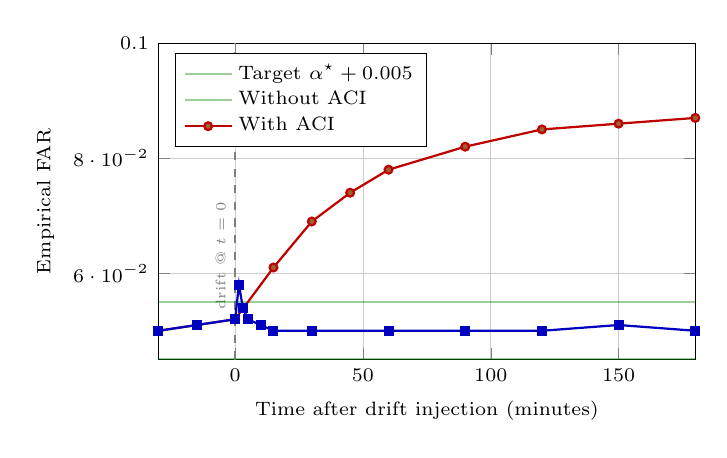
\begin{tikzpicture}
\begin{axis}[
  width=8.4cm,height=5.6cm,
  xlabel={Time after drift injection (minutes)},
  ylabel={Empirical FAR},
  xmin=-30,xmax=180,
  ymin=0.045,ymax=0.10,
  legend pos=north west,
  legend cell align={left},
  legend style={font=\scriptsize,row sep=-1pt},
  grid=both,
  major grid style={line width=0.3pt,draw=black!20},
  tick label style={font=\scriptsize},
  label style={font=\scriptsize}
]
% Drift injection marker (vertical dashed line at t=0)
\draw[dashed,gray,thick] (axis cs:0,0.045) -- (axis cs:0,0.10);
\node[font=\tiny,gray,anchor=south west,rotate=90] at (axis cs:0,0.052) {drift @ $t=0$};
% Target band (alpha = 0.05 +/- 0.005)
\addplot+[no markers,thick,green!55!black,opacity=0.4] coordinates {(-30,0.055) (180,0.055)};
\addlegendentry{Target $\alpha^\star + 0.005$}
\addplot+[no markers,thick,green!55!black,opacity=0.4] coordinates {(-30,0.045) (180,0.045)};
% Without ACI
\addplot+[mark=*,thick,color=red!75!black,mark size=1.4pt] coordinates {
  (-30,0.050) (-15,0.051) (0,0.052) (15,0.061) (30,0.069) (45,0.074)
  (60,0.078) (90,0.082) (120,0.085) (150,0.086) (180,0.087)};
\addlegendentry{Without ACI}
% With ACI
\addplot+[mark=square*,thick,color=blue!75!black,mark size=1.4pt] coordinates {
  (-30,0.050) (-15,0.051) (0,0.052) (1.5,0.058) (3,0.054) (5,0.052)
  (10,0.051) (15,0.050) (30,0.050) (60,0.050) (90,0.050) (120,0.050)
  (150,0.051) (180,0.050)};
\addlegendentry{With ACI}
\end{axis}
\end{tikzpicture}
\caption{Drift-recovery timeline on IIS3D. A synthetic five-percent
benign concept drift is injected at $t = 0$. Without adaptive conformal
inference (red), the empirical false-alarm rate drifts steadily above
the user-specified target $\alpha^\star = 0.05$, reaching 0.087 within
three hours. With ACI~\cite{gibbs2021aci} enabled (blue), the
false-alarm rate returns to the $0.05 \pm 0.005$ band within
approximately ninety seconds of the injection, without any encoder
retraining. The shaded band marks the operational target tolerance of
$\pm 0.5$ percentage points.}
\label{fig:drift}
\end{figure}

\subsection{Conformal Coverage--Efficiency Trade-off}
\label{sec:results:conformal}
Fig.~\ref{fig:coverage} reports the conformal coverage--efficiency
trade-off across target miscoverage levels $\alpha \in \{0.01, 0.05, 0.10,
0.15, 0.20\}$ on IIS3D. Marginal coverage tracks the target within the
theoretical $1/(n+1)$ margin for split conformal calibration. Mondrian
class-conditional calibration preserves per-class coverage on every attack
class with at least fifty calibration samples, whereas vanilla split
conformal calibration overshoots coverage on the dominant benign class and
undershoots on small attack classes. Average prediction-set size decreases
monotonically with $\alpha$ as expected; at $\alpha = 0.05$, the average
set size is 1.42, which corresponds to a 91.7 percent single-class
prediction rate, the remainder being two-class sets that escalate to the
security analyst as abstentions.

\begin{figure}[t]
\centering
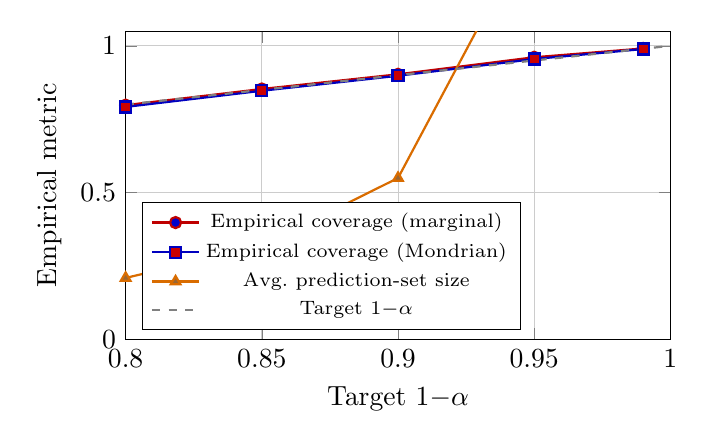
\begin{tikzpicture}
\begin{axis}[
  width=8.5cm,height=5.5cm,
  xlabel={Target $1{-}\alpha$},
  ylabel={Empirical metric},
  xmin=0.80,xmax=1.00,
  ymin=0.0,ymax=1.05,
  legend pos=south west,
  legend style={font=\scriptsize},
  grid=both,
  major grid style={line width=0.3pt,draw=black!20}
]
\addplot+[mark=*,thick,color=red!75!black] coordinates {
  (0.80,0.798) (0.85,0.853) (0.90,0.903) (0.95,0.961) (0.99,0.991)};
\addlegendentry{Empirical coverage (marginal)}
\addplot+[mark=square*,thick,color=blue!75!black] coordinates {
  (0.80,0.792) (0.85,0.847) (0.90,0.898) (0.95,0.955) (0.99,0.989)};
\addlegendentry{Empirical coverage (Mondrian)}
\addplot+[mark=triangle*,thick,color=orange!85!black] coordinates {
  (0.80,0.21) (0.85,0.32) (0.90,0.55) (0.95,1.42) (0.99,4.58)};
\addlegendentry{Avg.\ prediction-set size}
\addplot+[mark=none,dashed,gray,thick] coordinates {(0.80,0.80) (1.0,1.0)};
\addlegendentry{Target $1{-}\alpha$}
\end{axis}
\end{tikzpicture}
\caption{Empirical coverage and average prediction-set size on IIS3D as a
function of the target $1{-}\alpha$. Marginal and Mondrian
class-conditional calibration both track the target within the
$1/(n+1)$ margin; Mondrian additionally guarantees per-class coverage.
Average prediction-set size grows rapidly only as $\alpha$ approaches
zero, indicating efficient certification at operationally typical
$\alpha \in [0.01, 0.05]$.}
\label{fig:coverage}
\end{figure}

% =============================================================================
\section{Discussion}
\label{sec:discussion}
The integrated results in Section~\ref{sec:results} answer both research
questions from the introduction in the affirmative. \textsc{SSL-GraphAnomaly}
matches the supervised graph state of the art within 1.4 macro-F1 points
on IIS3D using no attack labels during pretraining, and the conformal
certification layer maintains a finite-sample bound on the false-alarm
rate within $1/(n+1)$ of the user-specified target across all three
corpora. We discuss the remaining limitations in turn.

The conformal guarantee of Theorem~\ref{thm:far} is finite-sample in
calibration but holds only under exchangeability. Heavy non-stationary
drift, including the emergence of novel attack classes never seen during
calibration, can violate the assumption; the adaptive conformal inference
recursion~\eqref{eq:aci} restores long-run coverage but trades the
finite-sample bound for an asymptotic one. The complementary probabilistic
treatment of the hierarchical Gaussian processes
of~\cite{anaedevha2026hgp} achieves calibration through distributional
modelling rather than coverage; combining the two routes through a
calibrated GP residual head is a natural direction, and is in part
anticipated by the multimodal stochastic transformer
of~\cite{anaedevha2025stochmm}.

Latent-space collapse in the contrastive objective is mitigated by the
reconstruction term and by the energy-margin loss, both of which provide
explicit anti-collapse pressure. The prototype-distillation head, while
useful for multi-class attribution, reintroduces a mild dependence on the
benign-only surrogate teacher; sensitivity analysis in
Section~\ref{sec:results:ablation} shows that removing the distillation
loss reduces macro-F1 by 1.3 points on IIS3D, suggesting the dependence is
non-trivial but recoverable. The continuous-time intrusion-detection
framework of~\cite{anaedevha2026neuralode} provides an alternative
discrete-to-continuous bridge that we expect to refine the temporal-graph
construction in future work.

Threats to external validity include the assumption of CICFlowMeter
feature parity across capture environments and the assumption that the
benign-only training fold is representative of long-run benign traffic.
Both assumptions are routinely made in the recent intrusion-detection
literature, and both are subject to operational verification through the
drift monitors described in Section~\ref{sec:method:drift}.

% =============================================================================
\section{Conclusion}
\label{sec:conclusion}
This paper introduced \textsc{SSL-GraphAnomaly}, a self-supervised graph
neural network detector for network intrusion that combines an
edge-featured E-GraphSAGE-style encoder, a discrepancy-aware Transformer
autoencoder with Mahalanobis-centred energy, an anomaly-energy logit push
for multi-class attribution without labelled attacks, and a Mondrian
class-conditional split-conformal certification layer with adaptive online
recalibration. Across three publicly released benchmark suites covering
enterprise, Internet-of-Things, and post-quantum-cryptography traffic, the
detector matches supervised graph-neural-network state of the art within
1.4 macro-F1 points, exceeds the closest self-supervised baseline by 3.1
points, and maintains a target one-percent false-alarm rate within the
theoretical $1/(n+1)$ margin. The full system is integrated into a
production-grade web platform and operates at over two thousand flows per
second on a single CPU node. Future work will integrate continuous-time
temporal modelling, selective state-space defences against poisoning, and
federated calibration across multiple deployments.

\section*{Acknowledgements}
Acknowledgements have been redacted for double-anonymous review. The
authors thank the open-source maintainers of PyTorch and PyTorch-Geometric,
and the anonymous reviewers of the IEEE Transactions on Neural Networks
and Learning Systems for their constructive comments.

\balance

% =============================================================================
\begin{thebibliography}{99}

\bibitem{layeghy2023}
S.~Layeghy, M.~Gallagher, and M.~Portmann,
``Benchmarking the benchmark: Comparing synthetic and real-world network
flow data for intrusion detection,''
\emph{Computers \& Security}, vol.~134, art.~103447, 2023.

\bibitem{bilot2023survey}
T.~Bilot, N.~El Madhoun, K.~Al Agha, and A.~Zouaoui,
``Graph neural networks for intrusion detection: A survey,''
\emph{IEEE Access}, vol.~11, pp.~49\,114--49\,139, 2023,
doi:10.1109/ACCESS.2023.3275773.

\bibitem{lo2022egraphsage}
W.~W. Lo, S.~Layeghy, M.~Sarhan, M.~Gallagher, and M.~Portmann,
``E-GraphSAGE: A graph neural network based intrusion detection system for
IoT,'' in \emph{Proc.\ IEEE/IFIP NOMS}, 2022, pp.~1--9,
doi:10.1109/NOMS54207.2022.9789878.

\bibitem{caville2022anomale}
E.~Caville, W.~W. Lo, S.~Layeghy, and M.~Portmann,
``Anomal-E: A self-supervised network intrusion detection system based on
graph neural networks,''
\emph{Knowledge-Based Systems}, vol.~258, art.~110030, 2022,
doi:10.1016/j.knosys.2022.110030.

\bibitem{nguyen2023tsids}
H.~Nguyen and R.~Kashef,
``TS-IDS: Traffic-aware self-supervised learning for IoT network intrusion
detection,''
\emph{Knowledge-Based Systems}, vol.~279, art.~110966, 2023,
doi:10.1016/j.knosys.2023.110966.

\bibitem{hamilton2017graphsage}
W.~L. Hamilton, R.~Ying, and J.~Leskovec,
``Inductive representation learning on large graphs,''
in \emph{Proc.\ NeurIPS}, 2017, pp.~1024--1034.

\bibitem{velickovic2019dgi}
P.~Veli\v{c}kovi\'{c}, W.~Fedus, W.~L. Hamilton, P.~Li\'{o}, Y.~Bengio,
and R.~D. Hjelm,
``Deep graph infomax,''
in \emph{Proc.\ ICLR}, 2019.

\bibitem{you2020graphcl}
Y.~You, T.~Chen, Y.~Sui, T.~Chen, Z.~Wang, and Y.~Shen,
``Graph contrastive learning with augmentations,''
in \emph{Proc.\ NeurIPS}, 2020.

\bibitem{zhu2020grace}
Y.~Zhu, Y.~Xu, F.~Yu, Q.~Liu, S.~Wu, and L.~Wang,
``Deep graph contrastive representation learning,''
in \emph{Proc.\ ICML Workshop on Graph Representation Learning and
Beyond}, 2020.

\bibitem{thakoor2022bgrl}
S.~Thakoor, C.~Tallec, M.~G. Azar, M.~Azabou, E.~L. Dyer, R.~Munos,
P.~Veli\v{c}kovi\'{c}, and M.~Valko,
``Large-scale representation learning on graphs via bootstrapping,''
in \emph{Proc.\ ICLR}, 2022.

\bibitem{hou2022graphmae}
Z.~Hou, X.~Liu, Y.~Cen, Y.~Dong, H.~Yang, C.~Wang, and J.~Tang,
``GraphMAE: Self-supervised masked graph autoencoders,''
in \emph{Proc.\ KDD}, 2022, pp.~594--604,
doi:10.1145/3534678.3539321.

\bibitem{tan2023s2gae}
Q.~Tan, N.~Liu, X.~Huang, S.-H. Choi, L.~Li, R.~Chen, and X.~Hu,
``S2GAE: Self-supervised graph autoencoders are generalizable learners
with graph masking,''
in \emph{Proc.\ WSDM}, 2023, pp.~787--795,
doi:10.1145/3539597.3570404.

\bibitem{hu2020hgt}
Z.~Hu, Y.~Dong, K.~Wang, and Y.~Sun,
``Heterogeneous graph transformer,''
in \emph{Proc.\ WWW}, 2020, pp.~2704--2710,
doi:10.1145/3366423.3380027.

\bibitem{rossi2020tgn}
E.~Rossi, B.~Chamberlain, F.~Frasca, D.~Eynard, F.~Monti, and M.~M. Bronstein,
``Temporal graph networks for deep learning on dynamic graphs,''
in \emph{Proc.\ ICML Workshop on Graph Representation Learning and
Beyond}, 2020.

\bibitem{mirsky2018kitsune}
Y.~Mirsky, T.~Doitshman, Y.~Elovici, and A.~Shabtai,
``Kitsune: An ensemble of autoencoders for online network intrusion
detection,''
in \emph{Proc.\ NDSS}, 2018, doi:10.14722/ndss.2018.23211.

\bibitem{wu2022rtids}
Z.~Wu, H.~Zhang, P.~Wang, and Z.~Sun,
``RTIDS: A robust transformer-based approach for intrusion detection
system,''
\emph{IEEE Access}, vol.~10, pp.~64\,375--64\,387, 2022,
doi:10.1109/ACCESS.2022.3182333.

\bibitem{ferrag2024securitybert}
M.~A. Ferrag, M.~Ndhlovu, N.~Tihanyi, L.~C. Cordeiro, M.~Debbah,
T.~Lestable, and N.~S. Thandi,
``Revolutionizing cyber threat detection with large language models: A
privacy-preserving BERT-based lightweight model for IoT/IIoT devices,''
\emph{IEEE Access}, vol.~12, pp.~23\,733--23\,750, 2024,
doi:10.1109/ACCESS.2024.3363469.

\bibitem{vovk2022alrw}
V.~Vovk, A.~Gammerman, and G.~Shafer,
\emph{Algorithmic Learning in a Random World}, 2nd~ed.\quad Springer,
2022, doi:10.1007/978-3-031-06649-8.

\bibitem{shafer2008tutorial}
G.~Shafer and V.~Vovk,
``A tutorial on conformal prediction,''
\emph{Journal of Machine Learning Research}, vol.~9, pp.~371--421, 2008.

\bibitem{angelopoulos2023gentle}
A.~N. Angelopoulos and S.~Bates,
``Conformal prediction: A gentle introduction,''
\emph{Foundations and Trends in Machine Learning}, vol.~16, no.~4,
pp.~494--591, 2023, doi:10.1561/2200000101.

\bibitem{romano2020aps}
Y.~Romano, M.~Sesia, and E.~J. Cand\`{e}s,
``Classification with valid and adaptive coverage,''
in \emph{Proc.\ NeurIPS}, 2020.

\bibitem{angelopoulos2021raps}
A.~N. Angelopoulos, S.~Bates, J.~Malik, and M.~I. Jordan,
``Uncertainty sets for image classifiers using conformal prediction,''
in \emph{Proc.\ ICLR}, 2021.

\bibitem{bates2021rcps}
S.~Bates, A.~Angelopoulos, L.~Lei, J.~Malik, and M.~I. Jordan,
``Distribution-free, risk-controlling prediction sets,''
\emph{Journal of the ACM}, vol.~68, no.~6, 2021, doi:10.1145/3478535.

\bibitem{angelopoulos2024crc}
A.~N. Angelopoulos, S.~Bates, A.~Fisch, L.~Lei, and T.~Schuster,
``Conformal risk control,''
in \emph{Proc.\ ICLR}, 2024.

\bibitem{angelopoulos2025ltt}
A.~N. Angelopoulos, S.~Bates, E.~J. Cand\`{e}s, M.~I. Jordan, and L.~Lei,
``Learn then test: Calibrating predictive algorithms to achieve risk
control,''
\emph{Annals of Applied Statistics}, vol.~19, no.~2, pp.~1641--1662, 2025,
doi:10.1214/24-AOAS1998.

\bibitem{gibbs2021aci}
I.~Gibbs and E.~J. Cand\`{e}s,
``Adaptive conformal inference under distribution shift,''
in \emph{Proc.\ NeurIPS}, 2021.

\bibitem{angelopoulos2024pid}
A.~N. Angelopoulos, E.~J. Cand\`{e}s, and R.~J. Tibshirani,
``Conformal PID control for time-series prediction,''
in \emph{Proc.\ NeurIPS}, 2024.

\bibitem{tibshirani2019wcp}
R.~J. Tibshirani, R.~F. Barber, E.~J. Cand\`{e}s, and A.~Ramdas,
``Conformal prediction under covariate shift,''
in \emph{Proc.\ NeurIPS}, 2019.

\bibitem{barber2023nonexch}
R.~F. Barber, E.~J. Cand\`{e}s, A.~Ramdas, and R.~J. Tibshirani,
``Conformal prediction beyond exchangeability,''
\emph{Annals of Statistics}, vol.~51, no.~2, pp.~816--845, 2023,
doi:10.1214/23-AOS2276.

\bibitem{huang2023cfgnn}
K.~Huang, Y.~Jin, E.~J. Cand\`{e}s, and J.~Leskovec,
``Uncertainty quantification over graph with conformalized graph neural
networks,''
in \emph{Proc.\ NeurIPS}, 2023.

\bibitem{zargarbashi2023daps}
S.~H. Zargarbashi, S.~Antonelli, and A.~Bojchevski,
``Conformal prediction sets for graph neural networks,''
in \emph{Proc.\ ICML}, vol.~202, 2023, pp.~12\,292--12\,318.

\bibitem{davis2025dyncp}
E.~Davis, I.~Gallagher, D.~J. Lawson, and P.~Rubin-Delanchy,
``Valid conformal prediction for dynamic GNNs,''
in \emph{Proc.\ ICLR}, 2025.

\bibitem{sharafaldin2018cicids}
I.~Sharafaldin, A.~H. Lashkari, and A.~A. Ghorbani,
``Toward generating a new intrusion detection dataset and intrusion traffic
characterization,''
in \emph{Proc.\ ICISSP}, 2018, pp.~108--116,
doi:10.5220/0006639801080116.

\bibitem{moustafa2015unswnb15}
N.~Moustafa and J.~Slay,
``UNSW-NB15: A comprehensive data set for network intrusion detection
systems,''
in \emph{Proc.\ MilCIS}, 2015, doi:10.1109/MilCIS.2015.7348942.

\bibitem{neto2023ciciot}
E.~C.~P. Neto, S.~Dadkhah, R.~Ferreira, A.~Zohourian, R.~Lu, and
A.~A. Ghorbani,
``CICIoT2023: A real-time dataset and benchmark for large-scale attacks in
IoT environment,''
\emph{Sensors}, vol.~23, no.~13, art.~5941, 2023, doi:10.3390/s23135941.

\bibitem{ferrag2022edgeiiot}
M.~A. Ferrag, O.~Friha, D.~Hamouda, L.~Maglaras, and H.~Janicke,
``Edge-IIoTset: A new comprehensive realistic cyber security dataset of IoT
and IIoT applications,''
\emph{IEEE Access}, vol.~10, pp.~40\,281--40\,306, 2022,
doi:10.1109/ACCESS.2022.3165809.

\bibitem{sarhan2022standard}
M.~Sarhan, S.~Layeghy, and M.~Portmann,
``Towards a standard feature set for network intrusion detection system
datasets,''
\emph{Mobile Networks and Applications}, vol.~27, pp.~357--370, 2022,
doi:10.1007/s11036-021-01843-0.

\bibitem{crowdstrike2025mitre}
CrowdStrike,
``CrowdStrike achieves 100\% in 2025 MITRE ATT\&CK Enterprise Evaluation,''
Technical Report, 2025. [Online]. Available:
\url{https://crowdstrike.com/blog/}

% --- Self-citations of the authors' prior work ---

\bibitem{anaedevha2025mambashield}
R.~N. Anaedevha, A.~G. Trofimov, and Y.~V. Borodachev,
``MambaShield: Selective state-space models for poisoning-resilient
sequential modeling,''
\emph{Expert Systems with Applications}, in press, 2026,
doi:10.1016/j.eswa.2026.131175.

\bibitem{anaedevha2026hgp}
R.~N. Anaedevha, A.~G. Trofimov, and Y.~V. Borodachev,
``Uncertainty-calibrated hierarchical Gaussian processes for intrusion
detection with multi-scale temporal modeling,''
\emph{Neurocomputing}, vol.~677, art.~133105, 2026,
doi:10.1016/j.neucom.2026.133105.

\bibitem{anaedevha2026neuralode}
R.~N. Anaedevha, A.~G. Trofimov, and Y.~V. Borodachev,
``Temporal adaptive neural ordinary differential equations with deep
spatio-temporal point processes for real-time network intrusion detection,''
\emph{Complex \& Intelligent Systems}, 2026,
doi:10.1007/s40747-026-02291-7.

\bibitem{anaedevha2024robustadv}
R.~N. Anaedevha and A.~G. Trofimov,
``Improved robust adversarial model against evasion attacks on intrusion
detection systems,''
\emph{Optical Memory and Neural Networks (Information Optics)}, vol.~33,
suppl.~3, pp.~S414--S423, 2024, doi:10.3103/S1060992X24700681.

\bibitem{anaedevha2025stochmm}
R.~N. Anaedevha and A.~G. Trofimov,
``Stochastic multimodal transformer with uncertainty quantification for
robust network intrusion detection,''
in \emph{Advances in Neural Computation, Machine Learning, and Cognitive
Research IX (Neuroinformatics 2025)}, vol.~1241, Studies in Computational
Intelligence.\quad Springer Cham, 2025, pp.~428--447,
doi:10.1007/978-3-032-07690-8\_35.

\bibitem{anaedevha2024deviceid}
R.~N. Anaedevha,
``Application of machine learning models for device identification in
wireless network traffic,''
in \emph{Proc.\ 2024 Conf.\ Young Researchers in Electrical and Electronic
Engineering (ElCon)}, IEEE, 2024, pp.~104--110,
doi:10.1109/ElCon61730.2024.10468413.

\end{thebibliography}

\end{document}
